\section{Push notifications and power management on iOS}
\label{sec:pushnotification}
\tbd{AL: this section is not intended to be as is in the final report,
but just a collection of results that can be incorporated in the final
document if needed.}

All the following experiments are performed on an iphone 4 with iOS
6.0.1.  At the beginning of each experiment we close all applications
and restart the iphone. The iphone is connected in wifi to a
controlled access point on which we perform a tcpdump on the wifi
interface and monitor the wifi association between the access point
and the iphone. Each experiment lasts for around 1 hour. 

In a first set of experiments, we consider a default iphone setting with
3G and wifi enabled, and the iphone unplugged. This corresponds to a
typical setting for a user on move. 




\begin{figure}
\centering
        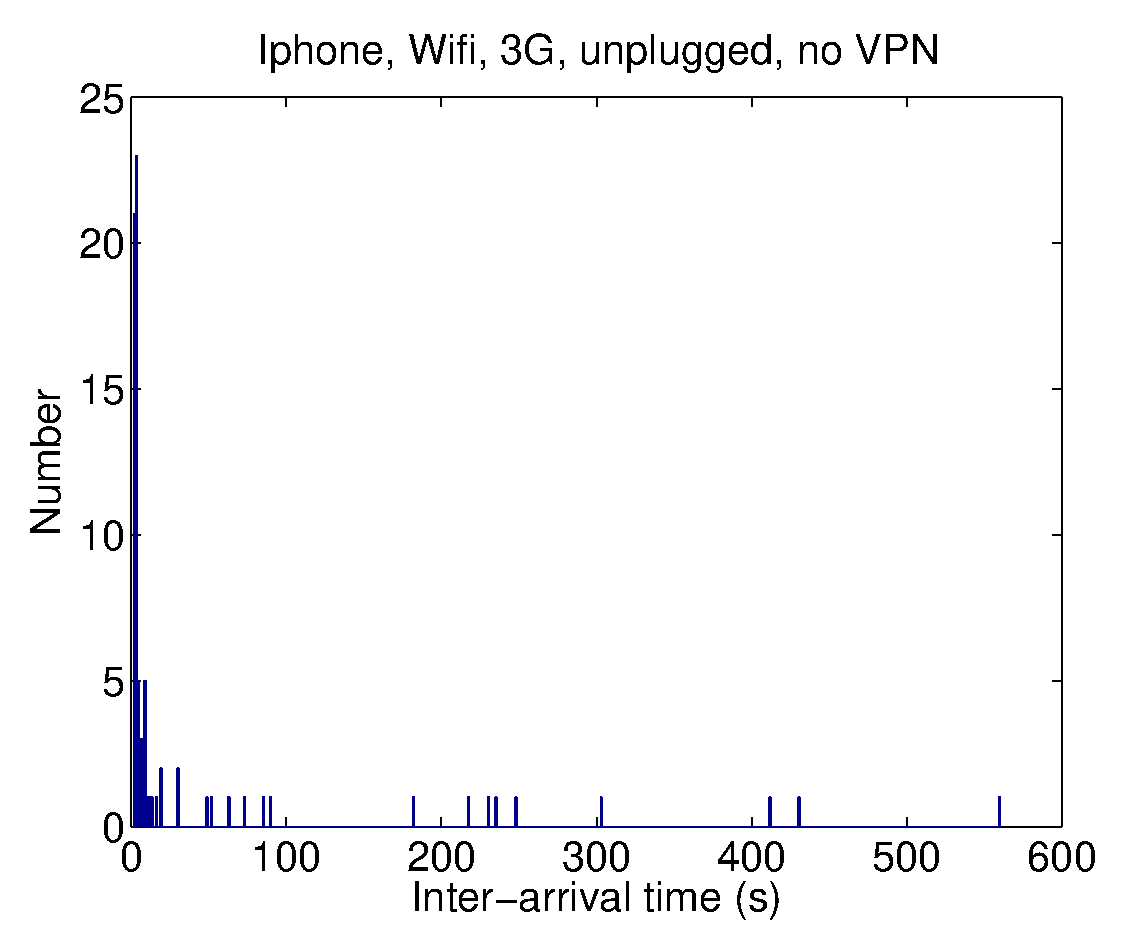
\includegraphics[width=0.8\linewidth]{../../code/pushNotification/Fig/bw_iphone_wifi_3g_unplug_novpn_interTs.eps}
  \caption{.}
  \label{fig:}
\end{figure}

\begin{figure}
\centering
        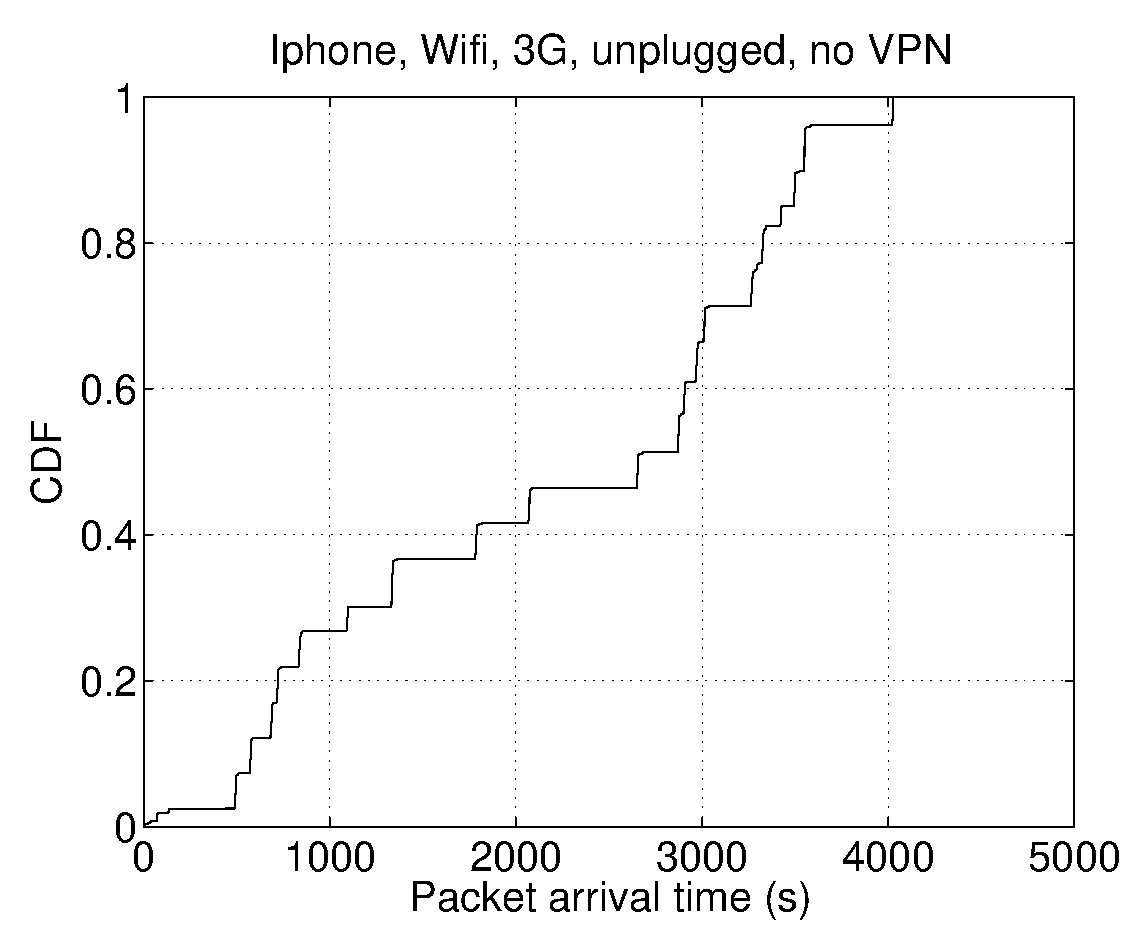
\includegraphics[width=0.8\linewidth]{../../code/pushNotification/Fig/bw_iphone_wifi_3g_unplug_novpn_ts.eps}
  \caption{.}
  \label{fig:}
\end{figure}

\begin{figure}
\centering
        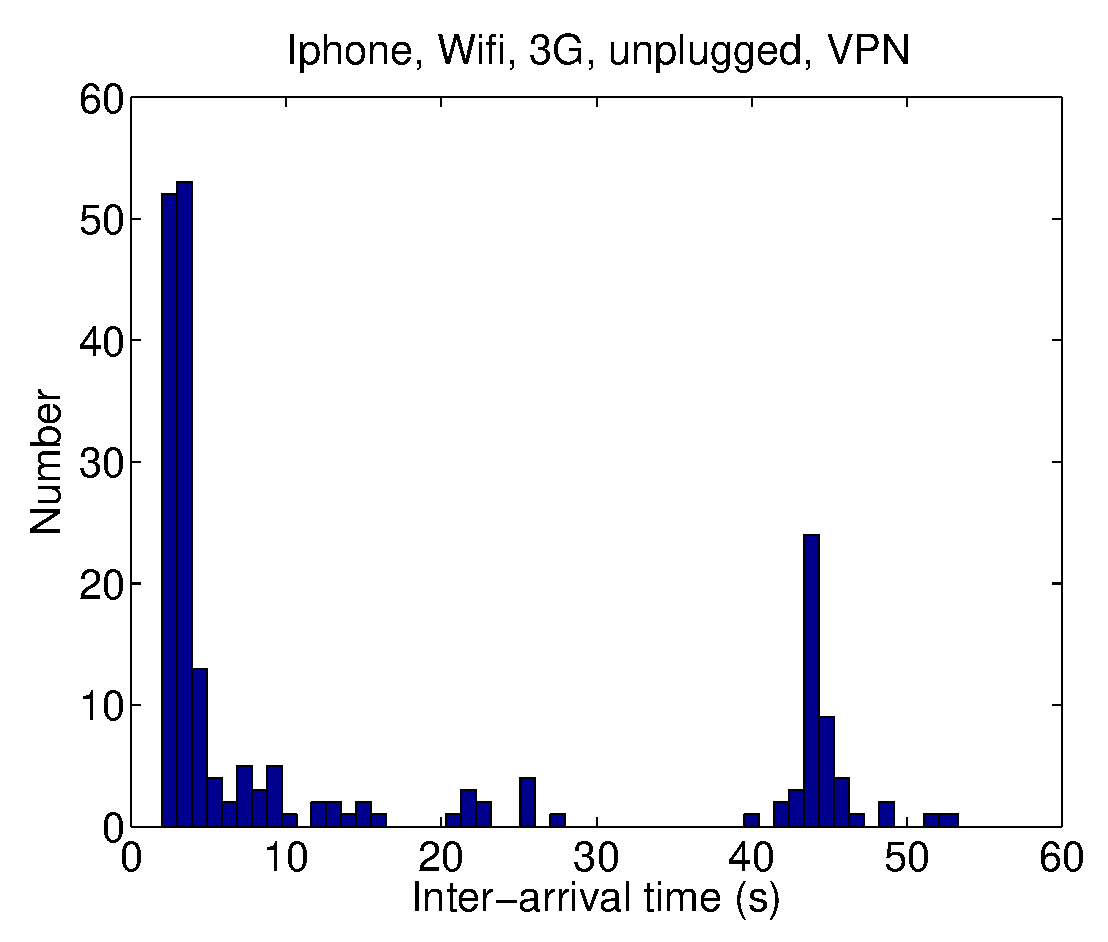
\includegraphics[width=0.8\linewidth]{../../code/pushNotification/Fig/bw_iphone_wifi_3g_unplug_vpn_interTs.eps}
  \caption{.}
  \label{fig:}
\end{figure}

\begin{figure}
\centering
        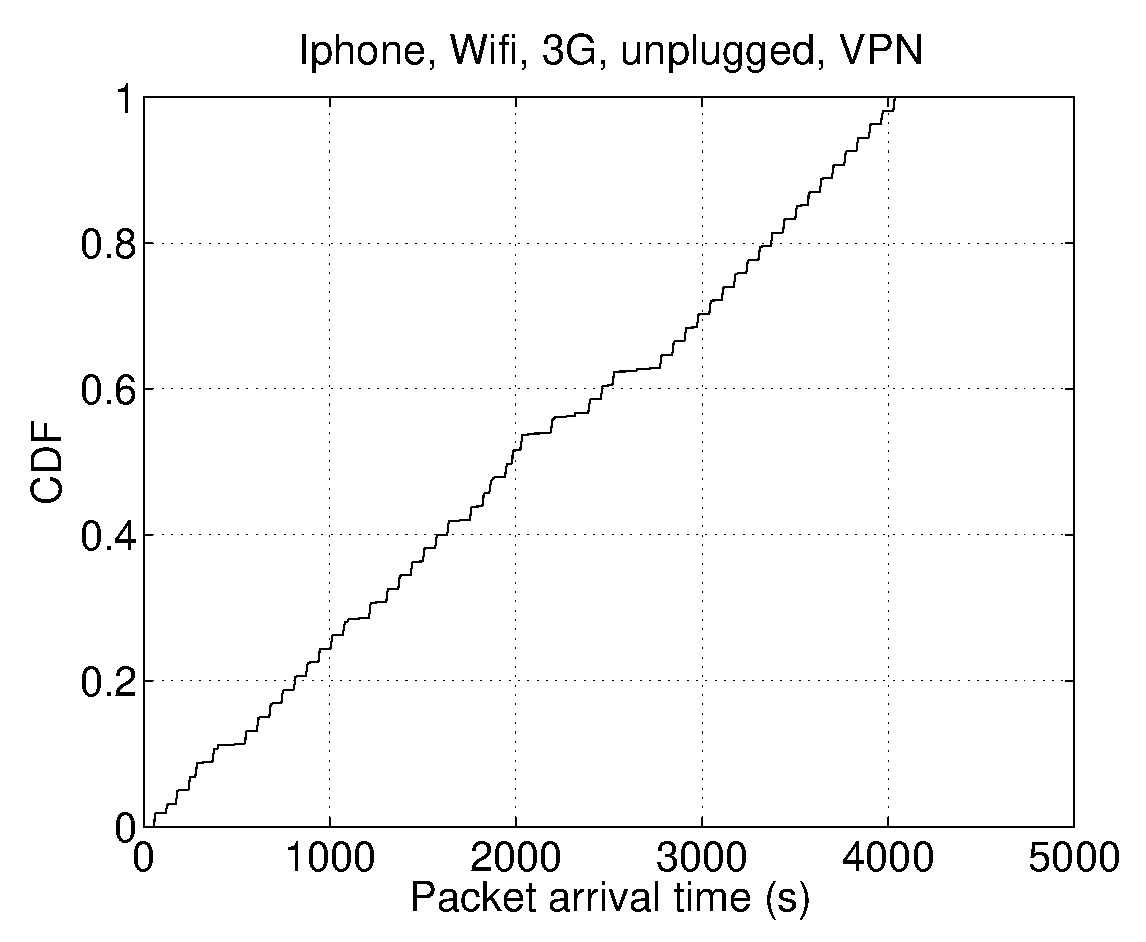
\includegraphics[width=0.8\linewidth]{../../code/pushNotification/Fig/bw_iphone_wifi_3g_unplug_vpn_ts.eps}
  \caption{.}
  \label{fig:}
\end{figure}

\begin{figure}
\centering
        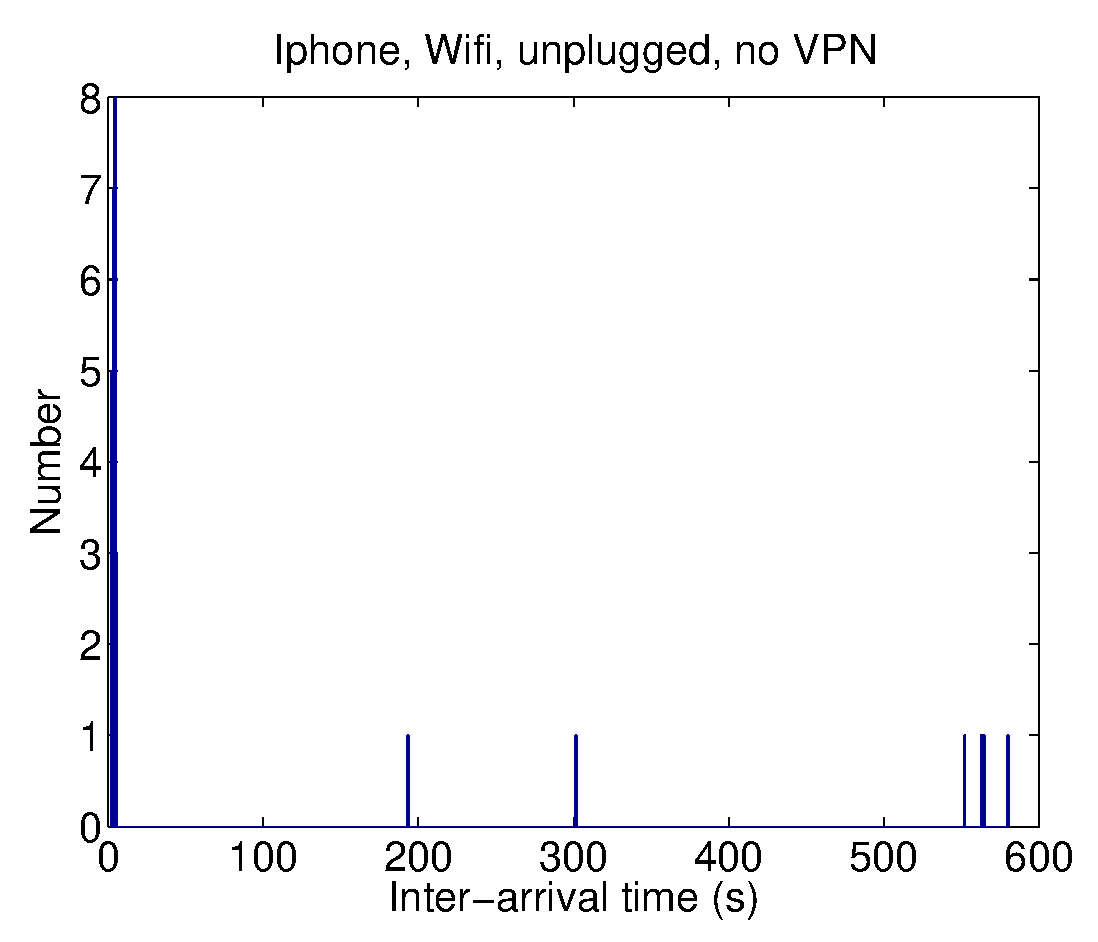
\includegraphics[width=0.8\linewidth]{../../code/pushNotification/Fig/bw_iphone_wifi_unplug_novpn_interTs.eps}
  \caption{.}
  \label{fig:}
\end{figure}

\begin{figure}
\centering
        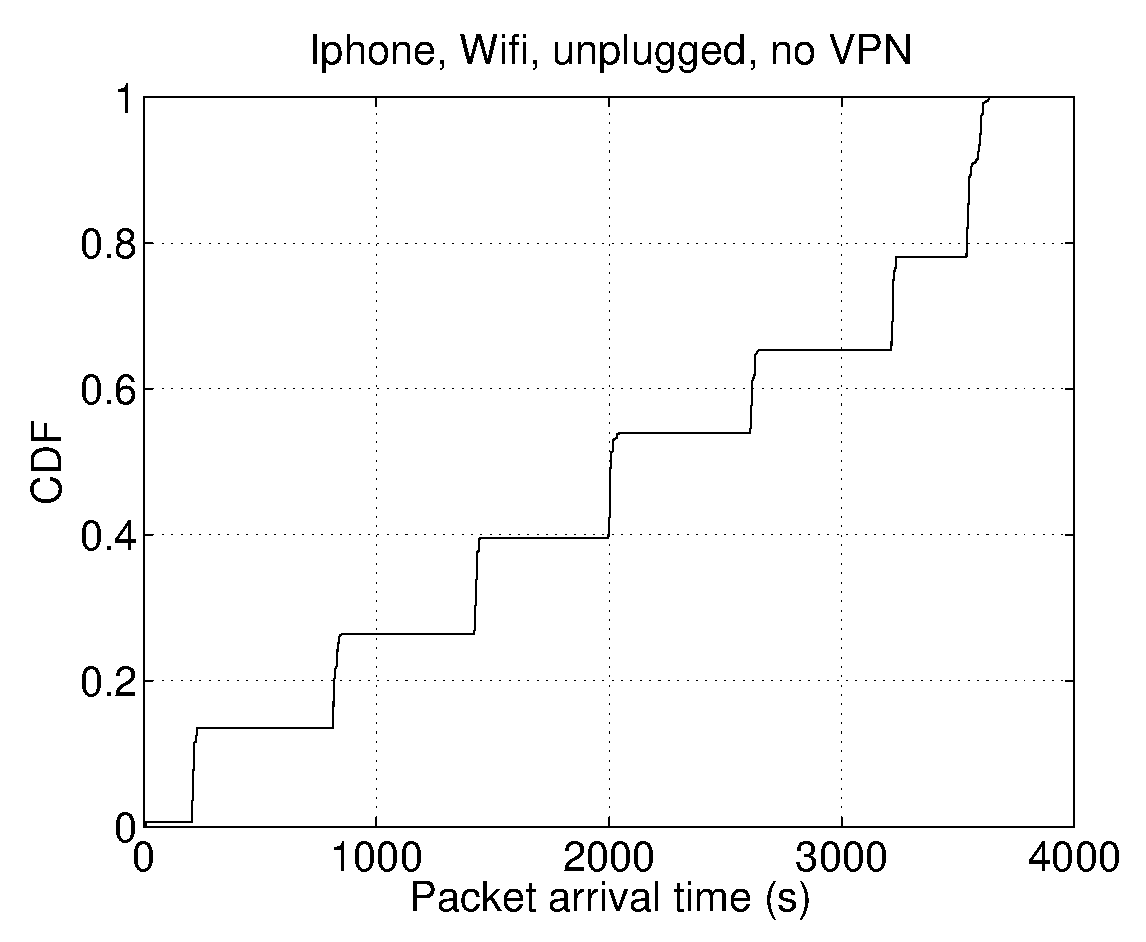
\includegraphics[width=0.8\linewidth]{../../code/pushNotification/Fig/bw_iphone_wifi_unplug_novpn_ts.eps}
  \caption{.}
  \label{fig:}
\end{figure}

\begin{figure}
\centering
        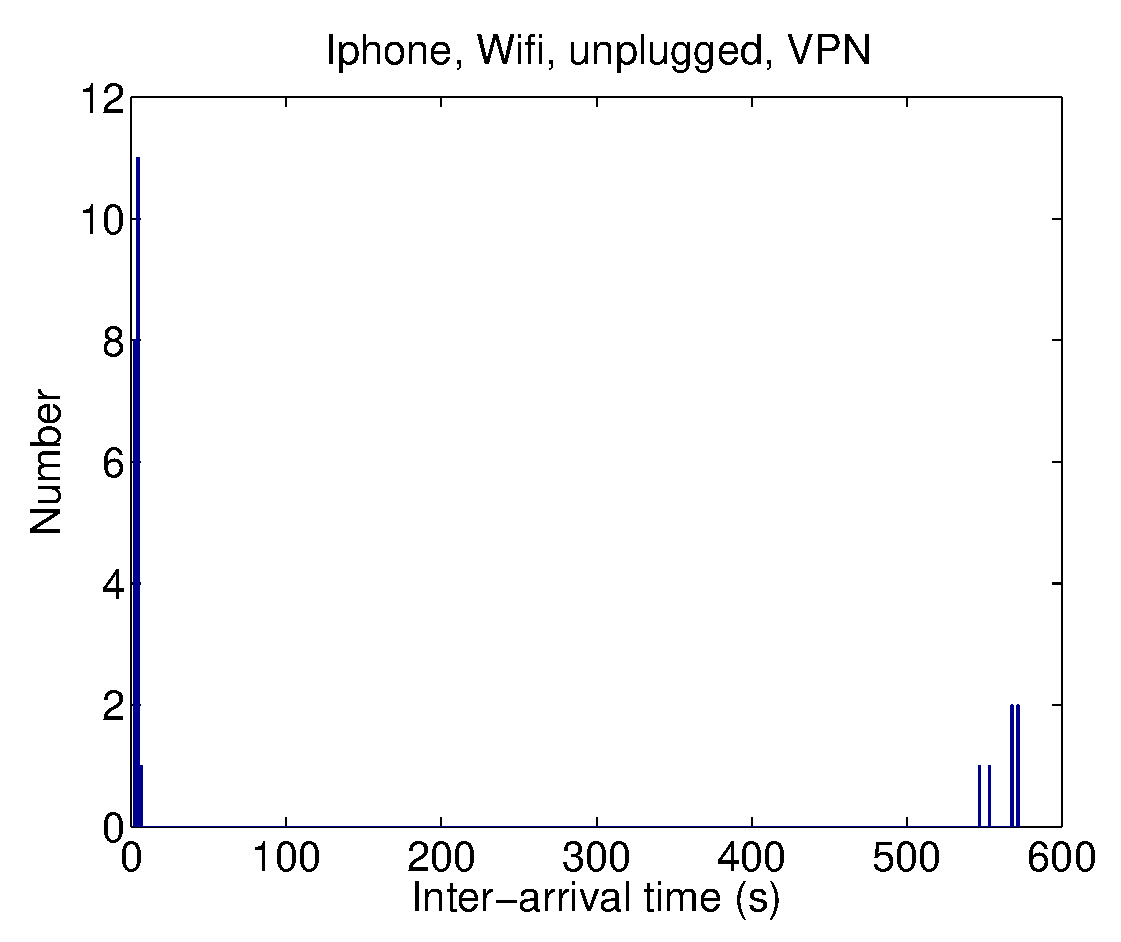
\includegraphics[width=0.8\linewidth]{../../code/pushNotification/Fig/bw_iphone_wifi_unplug_vpn_interTs.eps}
  \caption{.}
  \label{fig:}
\end{figure}

\begin{figure}
\centering
        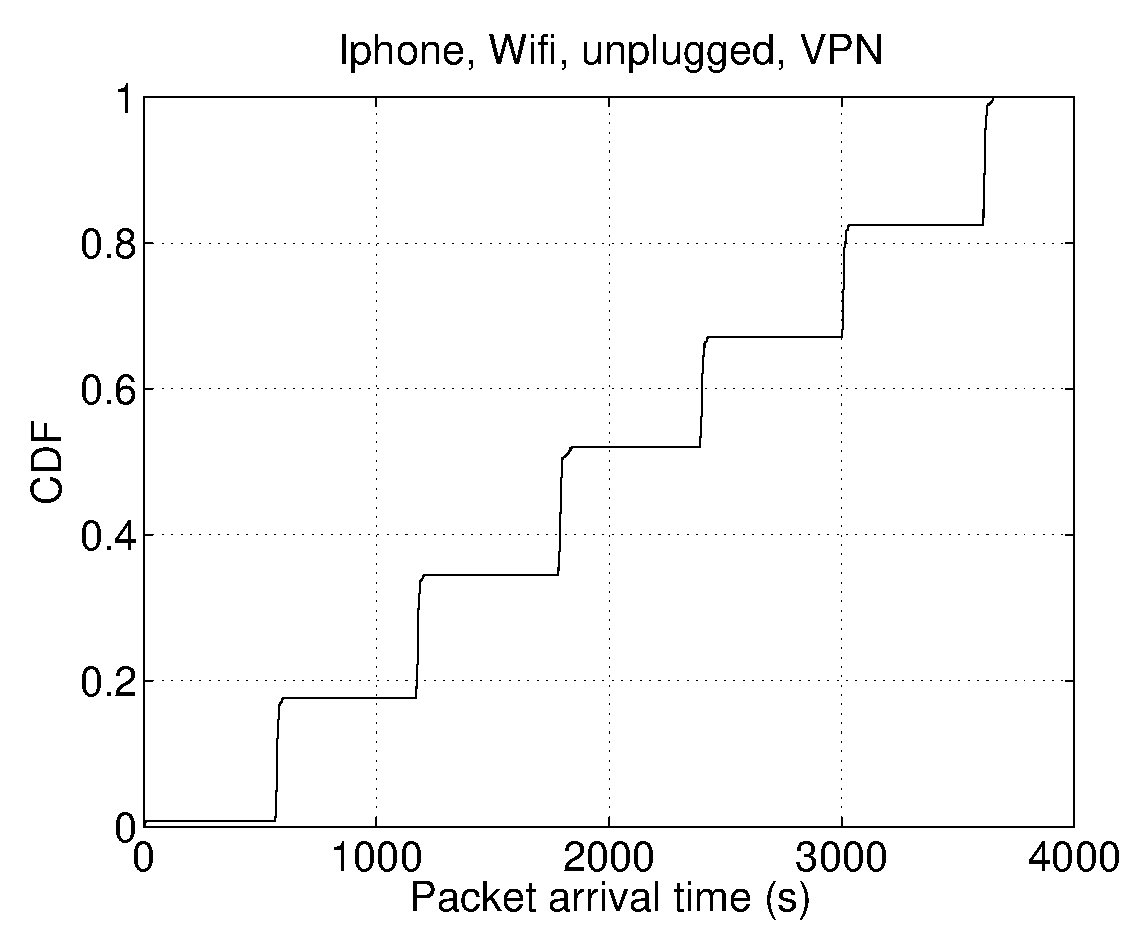
\includegraphics[width=0.8\linewidth]{../../code/pushNotification/Fig/bw_iphone_wifi_unplug_vpn_ts.eps}
  \caption{.}
  \label{fig:}
\end{figure}



%%% Local Variables: 
%%% mode: latex
%%% TeX-master: "main"
%%% End: 
